%% ============================================================
%% Stablecoin StressBench --- ICAIF 2026 Submission
%% ACM SIGCONF format, 8-page limit, double-blind anonymous
%% ============================================================
\documentclass[sigconf,anonymous,natbib=false]{acmart}

%% ---- Packages -----------------------------------------------
\usepackage{booktabs}
\usepackage{multirow}
\usepackage{graphicx}
\usepackage{amsmath}
\usepackage{microtype}
\usepackage{url}
\usepackage[T1]{fontenc}
\usepackage[utf8]{inputenc}
\usepackage{enumitem}

%% ---- ACM metadata -------------------------------------------
\acmConference[ICAIF '26]{ACM International Conference on AI in Finance}{November 14--17, 2026}{Milan, Italy}
\acmDOI{}
\acmISBN{}
\setcopyright{none}

%% ---- Spacing ---------------------------------------------------
\setlength{\emergencystretch}{3em}
\tolerance=1000
\hbadness=1500
\setlength{\textfloatsep}{8pt plus 2pt minus 2pt}
\setlength{\floatsep}{6pt  plus 2pt minus 2pt}
\setlength{\intextsep}{6pt  plus 2pt minus 2pt}
\setlength{\abovecaptionskip}{4pt}
\setlength{\belowcaptionskip}{1pt}
\setlength{\abovedisplayskip}{7pt plus 2pt minus 1pt}
\setlength{\belowdisplayskip}{7pt plus 2pt minus 1pt}
\setlength{\abovedisplayshortskip}{4pt plus 2pt}
\setlength{\belowdisplayshortskip}{5pt plus 2pt minus 1pt}

%% ---- Convenience macros ------------------------------------
\newcommand{\bps}{\,\text{bps}}
\newcommand{\task}[1]{\texttt{\small #1}}

%% =============================================================
\begin{document}

\title{Stablecoin StressBench: The Highest-AUROC Model Loses the Most
Money Under a \texorpdfstring{$12\times$}{12x} Execution Gap That Vanishes On-Chain}

%% ---- Abstract -----------------------------------------------
\begin{abstract}\sloppy
On 10 March 2023, Silicon Valley Bank's seizure forced USDC off its
dollar peg. Price charts showed $34.3\%$ of one-minute windows as
profitable stablecoin arbitrage; fewer than $3$ in $100$ ($2.88\%$)
survived VWAP book-walking, fees, and settlement, a \textbf{$12\times$
gap} between visible and executable profit (proxy-bounded to $12$--$14\times$
under a conservative $20\%$ depth haircut).  A model scoring well on
price labels can still lose money on every trade.
We release \textbf{Stablecoin StressBench}, an 18-event catalogue across
seven mechanism classes with per-minute VWAP (volume-weighted average
price) book-walking labels, route provenance, and a hindsight-oracle
ceiling (CC-BY~4.0), and use it to ask what works and what does not.
\emph{What does not work:} every calm-trained family we test (tabular,
sequence, reinforcement-learning, and change-point) loses money despite high
AUROC; the highest-AUROC model (GRU, $0.80$) is the largest loser ($-239\bps$),
a direct quantification of the AUROC--P\&L inversion under class imbalance.
A pre-registered $81$-path search over training protocols, feature sets, and
models finds \textbf{zero} paths that select profitable windows out-of-sample
under a Benjamini--Hochberg FDR($0.10$) gate; even purged in-event
cross-validation (train and test \emph{within} the SVB crisis) is strongly
negative ($-66$ to $-122\bps$), so executable-window \emph{selection} is
unsolved, not merely non-transferable.
\emph{What does work:} the barrier is venue-specific. On real on-chain
Curve/AMM data, where execution cost is the bounded pool slippage rather than
order-book impact, a simple deviation rule is profitable in $5/5$ episodes;
$4/5$ survive a conservative $30\bps$ gas haircut ($+169$ to $+463\bps$,
moving-block bootstrap $95\%$ CIs above zero), the lone exception being the
small USDC/SVB on-chain dislocation. The same signal that loses money on every
CEX path is capturable on-chain, so the optical-to-executable barrier is a
property of CEX order-book microstructure, not of stablecoin depegs.
\end{abstract}

\keywords{transfer learning, meta-labeling, reinforcement learning,
  execution-aware labels, market microstructure, stablecoin arbitrage,
  financial benchmarks}

\begin{CCSXML}
<ccs2012>
<concept><concept_id>10003752</concept_id>
<concept_desc>Applied computing~Economics</concept_desc>
<concept_significance>500</concept_significance></concept>
<concept><concept_id>10010147.10010257</concept_id>
<concept_desc>Computing methodologies~Machine learning</concept_desc>
<concept_significance>300</concept_significance></concept>
</ccs2012>
\end{CCSXML}
\ccsdesc[500]{Applied computing~Economics}
\ccsdesc[300]{Computing methodologies~Machine learning}

\maketitle

%% =============================================================
\section{Introduction}
\label{sec:intro}

Stablecoin stress is not one phenomenon but seven.
A \emph{stablecoin} is a cryptocurrency engineered to hold a fixed value---almost
always one US dollar---and serves as the dollar settlement rail of crypto markets;
when it loses that anchor (a \emph{depeg}), the event is at once a systemic-risk
shock and, on the price chart, an apparent arbitrage.
From 2020 to 2023 we catalogue 18 distinct depeg episodes spanning
algorithmic death spirals (Terra/LUNA, IRON/TITAN), fiat-reserve shocks
(USDC/SVB), regulatory winddowns (BUSD), exchange-credit collapses
(FTX, Celsius), DeFi pool imbalances (Curve/USDT), collateral
liquidations (DAI Black Thursday), and real-world-asset failures
(USDR, Acala).
Yet every prior study examines a single mechanism, and none asks the
question a trader actually faces. Of the price dislocations that appear
during stress, how many can be captured at a profit?

The answer is far fewer than the chart suggests.
When USDC slipped below \$1 during the March 2023 SVB crisis, Bitcoin
bought with USDC looked cheaper than the same Bitcoin priced in real
dollars, free money on a price chart.
In practice it rarely was.
By the time an order walked the book, the discount had narrowed. Taker
fees and settlement delay consumed the rest.
Only 2.88\% of one-minute windows survived all three costs, against
34.3\% that appeared dislocated, a $12\times$ gap between visible and
executable arbitrage.

We separate three layers of the same event.
\textbf{Layer~1 (optical)} is what the price chart shows. A stablecoin's
\emph{basis}, its deviation from \$1, appears positive, suggesting a
profitable arbitrage.
\textbf{Layer~2 (executable)} is what survives real execution.  A market
order does not fill at the quoted price. It consumes successive price
levels in the order book, and the resulting VWAP (volume-weighted average
price, $\bar{P}=\sum_i P_i Q_i / \sum_i Q_i$ across consumed levels)
worsens with size.  Layer~2 keeps only the minutes where the VWAP-filled
profit, after fees and settlement delay, is still positive.
\textbf{Layer~3 (captured)} is what a model can flag in advance.
Gap~1 (Layer~1$\to$2) is a measurement problem: price labels overstate
tradeable performance by $12\times$. Gap~2 (Layer~2$\to$3) is a training
problem: calm-trained models fail on unseen stress regimes. Layer-1-only
dislocations are \textbf{\emph{optical}}; survivors are \textbf{\emph{executable}}.
Figure~\ref{fig:framework} shows all three layers for the SVB test
window and traces one representative false-positive minute from
apparent profit to net loss.
Basis points (bps) are hundredths of a percent (100\,bps $=$ 1\%).

We establish each gap against a ground truth. Terra/LUNA, a mechanistically
independent algorithmic collapse, is our known reference (gap $5.9\times$,
$2.40\%$ executable) and supplies the cross-mechanism training signal; USDC/SVB,
a fiat-reserve shock with route-complete order-book depth, is the execution-grade
test case (gap $12\times$, $2.88\%$ executable, widening to $14\times$ under a
$20\%$ depth haircut). The same gap in two unrelated mechanisms makes the
phenomenon structural, not an artefact of either event; only the \emph{Tier-A}
execution labels, backed by real full-depth order-book data rather than a
price-only proxy, are SVB-specific.

No calm-trained model captures this gap. In stress the order book withdraws depth and
widens spreads, but \emph{which} dislocated minutes are executable turns out to be
unpredictable from that microstructure---we show below that even a model trained and
tested \emph{within} the SVB crisis cannot select them. The barrier is not the crisis,
it is the venue: on an automated market maker the same dislocation is capturable, because
execution cost is the bounded slippage of the pool invariant rather than open-ended
order-book impact.

\paragraph{Contributions}
\begin{enumerate}[leftmargin=*,itemsep=2pt,topsep=2pt]
  \item \textbf{An execution-aware benchmark that exposes a $12\times$ optical-to-executable gap.}
        StressBench supplies the apparatus: an 18-event source-tracked catalogue across seven
        mechanism classes, per-minute VWAP book-walking labels with route provenance, and a
        \emph{hindsight-oracle ceiling} that upper-bounds any model's profit. On the marquee
        USDC/SVB event, $34.3\%$ of minutes look dislocated but only $2.88\%$ are executable
        (a $12\times$ gap), so oracle capture---not price-label AUROC---is the right yardstick.
        (\S\ref{sec:benchmark}--\ref{sec:models})
  \item \textbf{The AUROC--P\&L inversion: executable-window selection is unsolved on the CEX order book.}
        Every calm-trained family loses money despite high AUROC, and the AUROC--P\&L relationship
        \emph{inverts}---we name this the \emph{AUROC--P\&L inversion}: the highest-AUROC model
        (GRU $0.80$) is the largest loser ($-239\bps$). A pre-registered
        $81$-path search (training protocols $\times$ feature sets $\times$ models) yields zero
        paths that clear a Benjamini--Hochberg FDR($0.10$) gate~\cite{benjamini1995fdr}; even
        purged in-event cross-validation is strongly negative, so the windows are unpredictable
        from this microstructure, not merely non-transferable. (\S\ref{sec:ladder},~\ref{sec:diagnostics})
  \item \textbf{What does work: the gap is venue-specific and the on-chain venue is tradeable.}
        On real on-chain Curve/AMM data, a simple deviation rule is profitable in $5/5$ episodes
        and $4/5$ survive a conservative $30\bps$ gas haircut ($+169$ to $+463\bps$, moving-block
        bootstrap CIs $>0$). The optical-to-executable barrier is therefore a property of CEX
        order-book microstructure---thin depth, taker fees, settlement delay---not of stablecoin
        depegs. (\S\ref{sec:venue},~\ref{sec:diagnostics})
\end{enumerate}

\paragraph{What you can do with this benchmark (CC-BY~4.0)}
The full catalogue, labels, oracle, and harness are released under CC-BY~4.0: test any
model against 18 real depeg episodes without data collection, measure oracle capture as a
principled denominator, and reproduce the $12\times$ gap from provided scripts.

Figure~\ref{fig:workflow} summarises the full benchmark pipeline, from
the 18-event catalogue through execution labels and the model ladder to
the released artefacts.

\begin{figure}[t]
  \centering
  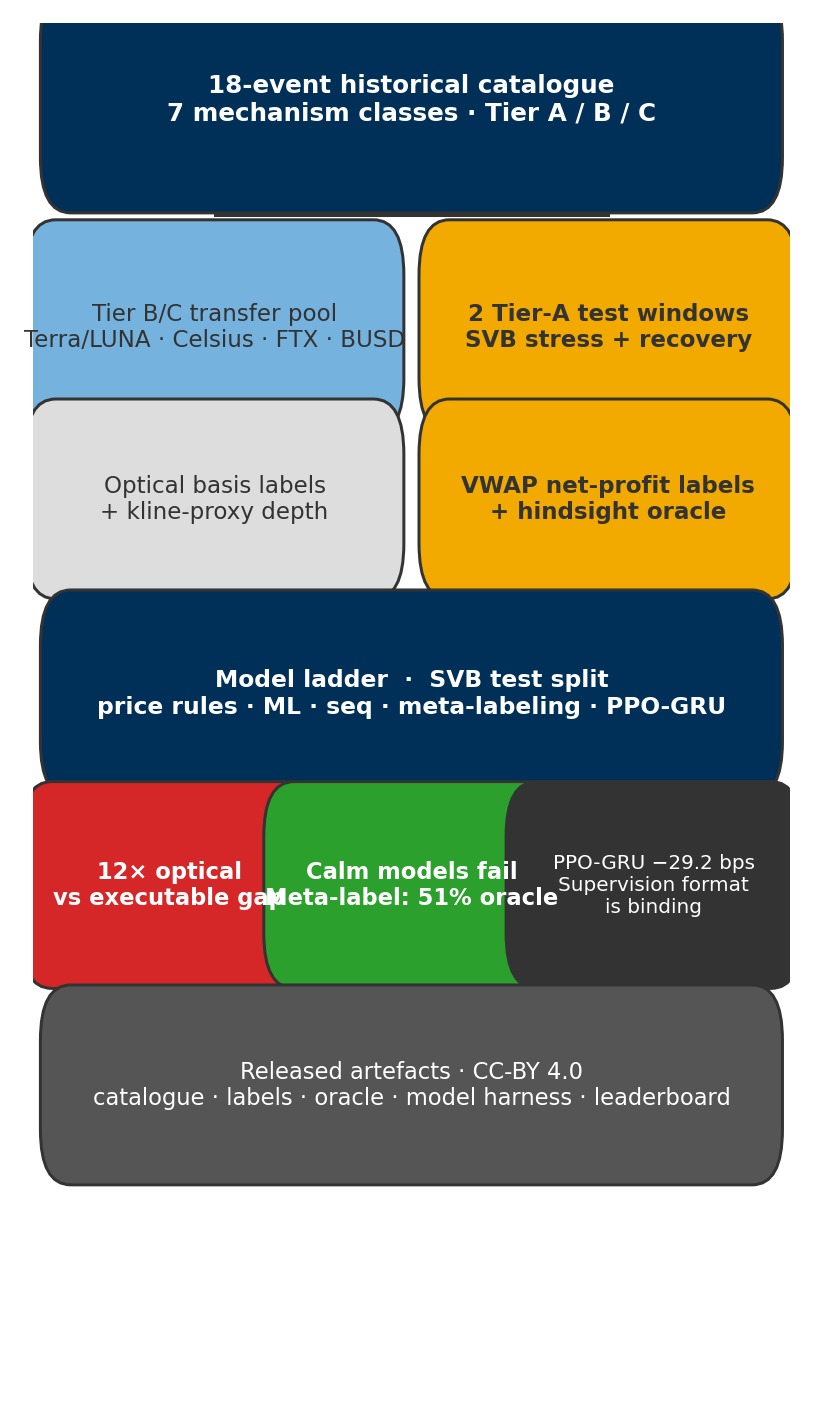
\includegraphics[width=0.72\columnwidth]{../results/paper_addon/figures/figure_workflow.png}
  \caption{StressBench pipeline. The 18-event catalogue is filtered to
    Tier-A execution-grade windows for VWAP labels and oracle evaluation;
    Tier-B/C events supply mechanism-diverse transfer training. Models are
    ranked by mean net bps per triggered trade, not price-label AUROC.}
  \label{fig:workflow}
\end{figure}


%% =============================================================
\section{Related Work}
\label{sec:related}

\textbf{Stablecoin stress and depeg detection.}
Uhlig \cite{uhlig2022luna} and Griffin and Shams \cite{griffin2020tether}
analyse Terra/LUNA and stablecoin non-fundamental demand.
Hernandez Cruz et al.\ \cite{hernandezcruz2024svb} study DEX liquidity
during the SVB collapse without modelling CEX execution costs.
Cintra and Holloway \cite{cintra2023bocpd} detect the Terra depeg
12 hours early via BOCPD on AMM reserves. We replicate their approach
on CEX cross-quote data and find AUROC~0.229, confirming that AMM
and CEX signals differ fundamentally.
None of these works provide VWAP-grade execution labels, a hindsight
oracle, or cross-mechanism transfer evaluation.  Our design therefore
follows three principles from the broader literature. Cont and
Kukanov~\cite{cont2013optimal} show VWAP book-walking is the correct
profitability measure for sequential execution, we implement this
exactly.  Shleifer and Vishny~\cite{shleifer1997limits} show that visible
arbitrage gaps need not survive execution frictions, our $12\times$ gap
is a direct measurement of this effect at one-minute resolution.  And
Lopez de Prado~\cite{lopezdeprado2018} shows that a meta-labeler trained
on the execution outcome outperforms direction predictors, our
cross-mechanism result is the evidence that this extends across stress
mechanisms.

\textbf{Limits to arbitrage and execution frictions.}
Shleifer and Vishny \cite{shleifer1997limits}, Gromb and Vayanos
\cite{gromb2010limits}, and Makarov and Schoar
\cite{makarov2020trading} show that visible price gaps need not be
profitable once execution frictions are included.
Our $12\times$ ratio is this effect measured at one-minute resolution.
Independent event-study evidence on the same episodes is consistent: crisis
arbitrage profitability falls from roughly $29\%$ to $7\%$ once fees and slippage
are applied~\cite{iaqf_uchicago_crosscurrency_2026}, and most apparent dislocations
sit outside executable bands~\cite{iaqf_nyu_spread_2026}.
Hautsch et al.\ \cite{hautsch2018blockchain} quantify settlement latency
as a first-order cost on blockchain assets.
Cont and Kukanov \cite{cont2013optimal} establish VWAP book-walking
as the correct profitability measure.
Gogol et al.\ \cite{gogol2024amm} measure Maximal Arbitrage Value on
AMM-to-CEX routes. Their partial execution labels cover AMM venues
only and lack a hindsight oracle.
Adams et al.\ \cite{adams2023mev} study swap costs on Uniswap without
stress-event execution analysis.

\textbf{ML and RL for execution.}
Lopez de Prado~\cite{lopezdeprado2018} introduces \emph{meta-labeling}. A
two-stage architecture in which a primary model (here, the Layer-1 dislocation
flag) proposes candidate trades, and a secondary \emph{meta-labeler} learns
which of those proposals will actually be profitable.  The meta-labeler thus
predicts the binary label ``this candidate survives execution'' rather than
predicting the market direction from scratch.  We extend this to the
\emph{cross-mechanism} setting, where the meta-labeler is trained on one crisis
type (Terra/LUNA) and applied unchanged to another (USDC/SVB).
Moallemi and Wang~\cite{moallemi2022rl} and Ning et al.~\cite{ning2021ddql}
supply the finite-horizon MDP framing we adopt for the RL baseline.
Mohl et al.\ \cite{jaxmarlhft2024} and Olby et al.\
\cite{rightplace2024} operate in reactive LOB environments with
market-impact feedback. Our diagnostic uses historical replay
without feedback, isolating training supervision as the variable.


%% =============================================================
\section{Benchmark Design}
\label{sec:benchmark}

\subsection{Data Sources and Instruments}
\label{sec:data}

The 18-event catalogue defines the historical stress universe. The
six-window empirical panel (56,134 one-minute bars) defines the model
dataset, and the Tier-A SVB windows define the execution-grade testbed.
Price features are sourced from Binance Vision (klines and aggTrades)
and Coinbase REST candles.
Net-profit labels use three depth legs across two centralised
exchanges (CEXs, i.e. Binance and Coinbase). The legs are Binance BTC-USDC (buy),
Binance BTC-USDT (sell), and Coinbase BTC-USD (reference).
The BTC-USDC buy leg uses kline-proxy depth for the SVB window because
the perpetual contract did not exist on Binance until January 2024.
A 20\% depth haircut confirms robustness (gap widens to $14\times$,
oracle stays above $+130\bps$).

Data quality varies by leg, and every record carries a provenance tag
(Table~\ref{tab:route_provenance}).

\begin{table}[t]
\centering
\caption{Route-leg depth provenance.}
\label{tab:route_provenance}
\setlength{\tabcolsep}{2pt}
{\scriptsize
\begin{tabular}{lp{2.1cm}p{2.1cm}}
\toprule
\textbf{Leg} & \textbf{SVB Mar~2023} & \textbf{2024 windows}\\
\midrule
Buy BTC-USDC    & kline-proxy$^\dagger$  & real L2 (futures)\\
Cross USDC-USDT & partial/proxy, real L2 where archived  & real L2 (futures)\\
Sell BTC-USDT   & raw/futures depth     & real L2 (futures)\\
Ref BTC-USD     & candle-proxy          & candle-proxy\\
\bottomrule
\end{tabular}
}
{\footnotesize $^\dagger$BTC-USDC perpetual listed Jan~2024.
All 2022 windows kline-proxy.}
\end{table}

\begin{table}[t]
\centering
\caption{Dataset splits (56,134 one-minute bars).}
\label{tab:dataset}
\setlength{\tabcolsep}{4pt}
{\small
\begin{tabular}{llrr}
\toprule
\textbf{Split} & \textbf{Event} & \textbf{Min.} & \textbf{Pos.}\\
\midrule
Train      & Calm control ($\times$3) & 28,776 & 0.00\%\\
Validation & Terra/LUNA May~2022      & 11,526 & 2.30\%\\
Test       & USDC/SVB Mar~2023        & 15,832 & 2.88\%\\
\bottomrule
\end{tabular}
}
\end{table}

\subsection{Event-Based Split Design}
\label{sec:splits}

Splits are defined by event identity, so no model trained on the calm
split has encountered stress dynamics.
Threshold calibration uses the Terra/LUNA validation split, an
independent stress event, so the SVB test split is never observed
during model development.
The 2.88\% positive rate in the test split (Table~\ref{tab:dataset}) implies severe class imbalance.
We therefore report economic net bps as the primary criterion. AUROC
and AUPRC are secondary metrics.

Five leakage checks confirm validity. Label shuffles produce negative P\&L.
Lookahead does not improve performance. Train and test are separated by event identity.

The full 18-event catalogue with per-event mechanism taxonomy and Tier
classifications is available in the project repository.

\subsection{Benchmark Positioning}
\label{sec:positioning}
No prior benchmark (\S\ref{sec:related}) combines per-minute executable CEX
labels, route-level L2 provenance, a hindsight oracle ceiling, and
cross-mechanism transfer evaluation; StressBench provides all four.

\paragraph{Feature sets} Four nested sets (\texttt{price\_only} $\subset$
\texttt{price\_plus\_book} $\subset$ \texttt{price\_book\_frag} $\subset$
\texttt{price\_book\_settle}) isolate marginal signal from price basis,
microstructure (spread, depth, imbalance), fragmentation, and on-chain settlement
proxies (kline-proxy for SVB/Terra windows, Tier~B).


%% =============================================================
\section{Execution-Aware Labels}
\label{sec:labels}

\subsection{Three-Layer Framework}
\label{sec:framework}

Figure~\ref{fig:framework} structures the paper's central argument
visually, instantiating the three layers and two gaps defined in
\S\ref{sec:intro}: both gaps are nonzero, independent, and large.
Panel~(b) traces one representative false-positive minute through the
full cost stack, showing why 34.3\% optical activity collapses to
2.88\% executable.

\begin{figure}[t]
  \centering
  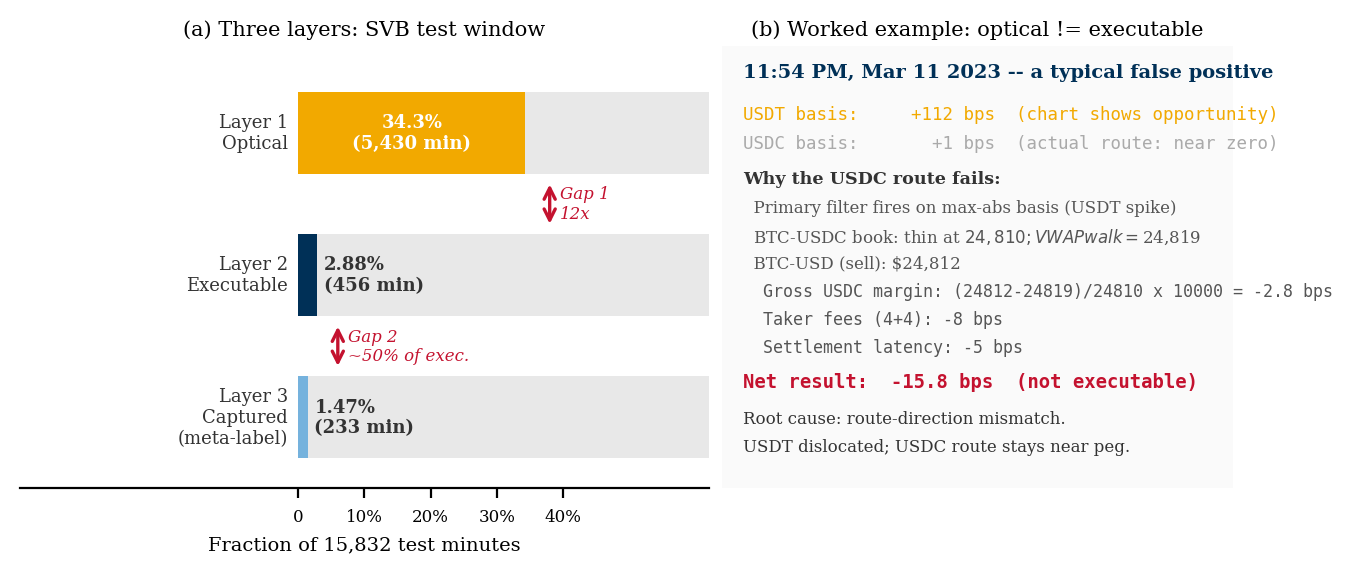
\includegraphics[width=\columnwidth]{../results/paper/figures/figure_framework.png}
  \caption{(a)~Three-layer framework for the SVB test window (15,832 min).
    Layer~1 optical (34.3\%), Layer~2 executable (2.88\%), Layer~3
    captured by cross-mechanism meta-labeling (1.47\%).
    Gap~1 ($12\times$) is a measurement problem. Gap~2 is a training problem.
    (b)~Worked example. A minute that appears profitable on the chart
    nets $-15.8\bps$ after VWAP book-walking, fees, and route-direction
    mismatch.}
  \label{fig:framework}
\end{figure}

\begin{figure}[t]
  \centering
  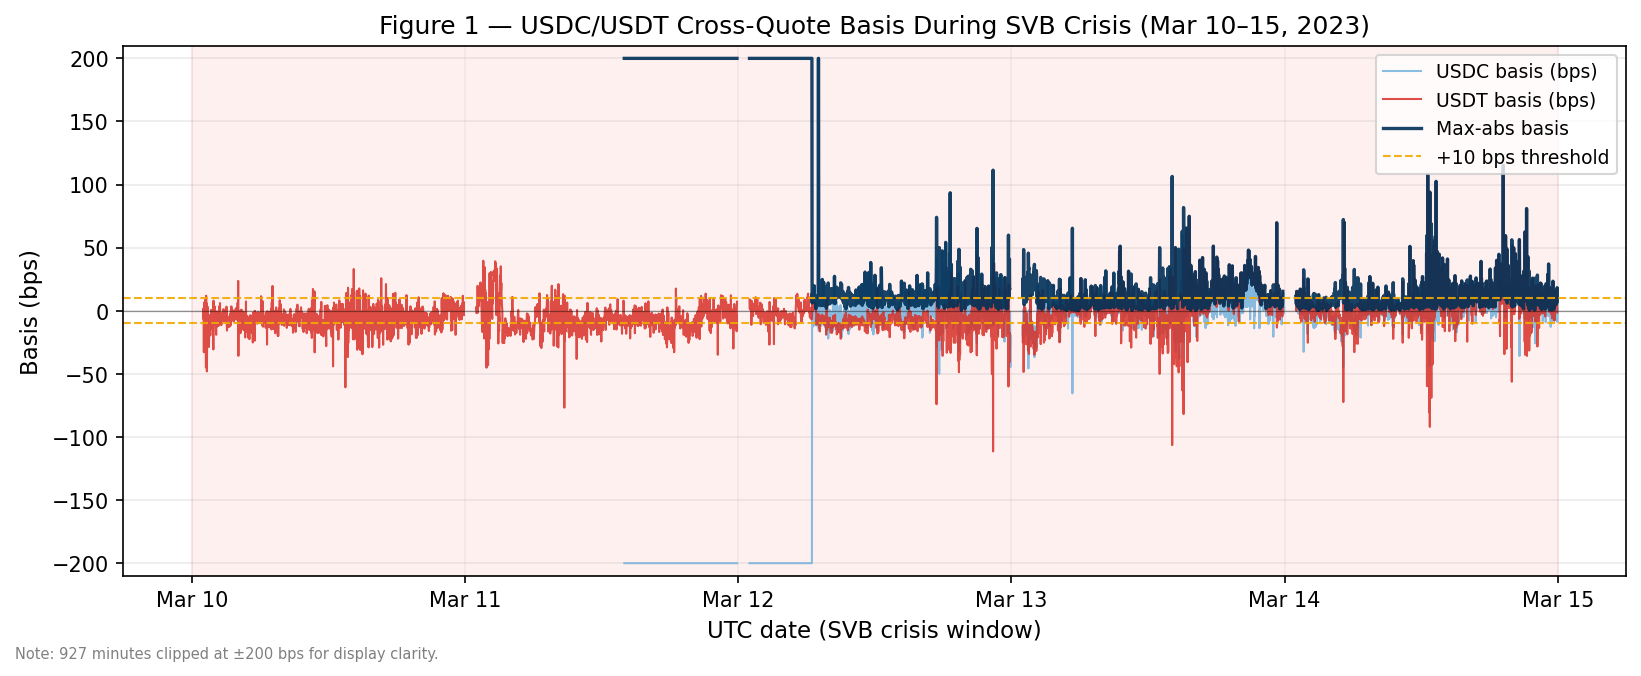
\includegraphics[width=\columnwidth]{../results/paper/figures/figure_1_usdc_basis_svb.png}
  \caption{Cross-quote basis during the SVB test window (Mar 10--20 2023).
    USDC basis (navy) exceeds 10\,bps in 12.4\% of minutes,
    USDT basis (red) in 27.4\%, and max-abs (gold) in 34.3\%.
    The price-to-execution ratio is $12\times$ (0\% depth haircut; $14\times$ under a 20\% haircut).}
  \label{fig:basis}
\end{figure}

\subsection{Cross-Quote Basis and Labels}
\label{sec:basis}

The cross-quote basis is the percentage gap between BTC priced in
a stablecoin (e.g. BTC-USDC) and BTC priced in real dollars
(BTC-USD on Coinbase). A non-zero basis signals an apparent
dislocation (Figure~\ref{fig:basis} shows it across the SVB window).
Three equations define the label construction.
\begin{align}
  b_{\text{USDC}}(t)  &\;=\; 10{,}000 \times
      \frac{P_{\text{BTC/USDC}}(t) - P_{\text{BTC/USD}}(t)}
           {P_{\text{BTC/USD}}(t)}
      \quad [\text{bps}] \label{eq:basis}\\[2pt]
  b_{\max}(t)         &\;=\; \max\!\left(
      |b_{\text{USDC}}(t)|,\;|b_{\text{USDT}}(t)|\right)
      \label{eq:bmax}\\[2pt]
  y_{\text{basis}}(t) &\;=\; \mathbf{1}\!\left[
      |b_{\text{USDC}}(t{+}h)| > \tau\right]
      \label{eq:ylabel}
\end{align}
Here $\mathbf{1}[\cdot]$ is the indicator function; the primary task is \task{basis\_usdc\_1m\_gt10bps} ($\tau{=}10\bps$, $h{=}1$\,min).

\subsection{VWAP Execution and Net Profit Labels}
\label{sec:netlabels}

\begin{equation}
  \text{net}(q,t) \;=\; 10{,}000 \times
    \left[\,
      \frac{\text{VWAP}_{\text{sell}} - \text{VWAP}_{\text{buy}}}{P_{\text{ref}}}
      - f_{\text{buy}} - f_{\text{sell}} - \delta_{\text{settle}}
    \,\right]
  \label{eq:net}
\end{equation}

\begin{equation}
  y_{\text{arb}}(q,h,t) \;=\; \mathbf{1}\!\left[\;
    \underset{s\,\in\,[t,\;t{+}h]}{\max} \text{net}(q,s) \;>\; c
  \;\right]
  \label{eq:yarb}
\end{equation}

Profit threshold $c{=}10\bps$, taker fee $4\bps$ per side, and
$\delta{=}5\bps$.
The $\delta$ assumption is validated against 100K on-chain USDC
ERC-20 transfers. Median cost was 1.4--3.2\,bps on nine of ten SVB
days. The one exception (Mar~11 gas spike) saw P95 reach 8.6\,bps.
\begin{equation}
  \text{Oracle}(q) \;=\; \frac{1}{|\mathcal{T}^+|}
    \sum_{t \in \mathcal{T}^+} \!\text{net}(q,t),\qquad
  \mathcal{T}^+ = \bigl\{t : \text{net}(q,t) > c\bigr\}
  \label{eq:oracle}
\end{equation}
The oracle is a hypothetical strategy that trades every
profitable window with perfect hindsight and represents an upper bound
no deployable model can exceed.
Oracle capture $\kappa_M = \bar{r}_M / \text{Oracle}(q)$ is the
fraction of the oracle's per-trade return recovered by model~$M$.


%% =============================================================
\section{Models and Evaluation}
\label{sec:models}

\subsection{Model Ladder}
\label{sec:stack}

The ladder is a sequential elimination experiment with one result at
every rung. Every family fails for the same reason, distributional
mismatch between calm training and stress test.

\textit{Architecture.} No help.
The GRU posts the highest AUROC among sequence models (0.80) and
the worst economic return ($-239\bps$, Figure~\ref{fig:auroc_pnl}).
Discriminability does not translate to profit at 2.88\% positive rate.

\textit{Feature engineering.} No help.
All four nested feature sets produce negative returns.
Depth and settlement signals offer no lift when the training split
contains zero stress-regime examples.

\textit{Class balancing.} No help.
Cost-sensitive reweighting cannot synthesise stress dynamics from calm
data. The issue is distributional, not proportional.

\textit{Regression targeting.} No help.
ExpNetProfitRegressor optimises the economic criterion directly and
reaches $-73.8\bps$. Label mismatch is not the explanation.

\textit{Regime detection.} No help.
Bayesian Online Change Point Detection (BOCPD), CUSUM, and EWMA all fail:
CEX basis is mean-reverting, not change-point structured (AUROC~0.229).

\textit{RL reward optimisation.} No help at identical density.
A conditioned PPO-GRU at 17\% primary-signal density earns
$-29.2\bps$. The reward signal is not a substitute for explicit
labels even when positive-example density is matched.

The cross-mechanism extension of meta-labeling operates in three steps.
Meta-labeling \cite{lopezdeprado2018} is a two-step filter. A cheap
rule flags candidate minutes, then a learned classifier keeps only the
ones likely to survive execution.
\begin{enumerate}[leftmargin=*,itemsep=1pt,topsep=2pt]
  \item \textbf{Primary filter.} Flag $t$ if
        $|b_{\text{USDC}}(t)|>\tau_1$ ($\tau_1{=}10\bps$).
  \item \textbf{Secondary classifier.} Fit $f_\theta$ on
        $\{(x_t,\,y_{\text{arb}}(t))\}_{t\in\mathcal{E}_{\text{train}}}$,
        where $\mathcal{E}_{\text{train}}$ is a mechanistically distinct
        stress event.
  \item \textbf{Entry.} Signal at $t$ iff primary fires
        and $f_\theta(x_t)>\theta^*$, where
        $\theta^* = \arg\max_\theta \sum_{i:\hat{p}_i>\theta}
        \text{net}(q,t_i)$ on the Terra/LUNA calibration block.
\end{enumerate}

\subsection{RL Execution Policy Baseline}
\label{sec:rl_baseline}

The entry-timing problem is framed as a finite-horizon MDP.
At each minute $t$ the agent observes the 30-step lookback of
\texttt{price\_plus\_book} features, selects
$a_t \in \{\texttt{enter},\texttt{wait}\}$, and receives reward
$r_t = \text{net}(q,t)$ on entry, 0 on wait.
We train a PPO agent with a GRU policy network (64 units, 30-step
lookback) using the cross-mechanism protocol, training on Terra/LUNA
stress windows only and evaluating on USDC/SVB without retraining.
This directly tests whether the sequential timing framing overcomes
the distributional mismatch that defeats all calm-trained models.

\subsection{Calibration and Evaluation}
\label{sec:eval}

Net bps denotes mean net basis points per triggered trade after VWAP,
taker fees, and settlement penalties.
Thresholds are calibrated on the validation split by maximising
$\theta^* = \arg\max_\theta \sum_{i:\hat{p}_i>\theta} \text{net}(q,t_i)$
over a 60-point linear grid on $[0.05, 0.95]$, subject to a minimum of 25 trades.
Primary metrics are mean net bps per triggered trade and oracle
capture $\kappa_M$.
Secondary metrics are AUROC and AUPRC.
NoTrade at $0\bps$ is the economic floor.

\textbf{Positive density clarification.}
Three densities appear: 2.88\% (executable fraction of SVB test minutes), 2.30\%
(executable fraction of the full Terra/LUNA stream), and 17\% (executable fraction
of \emph{primary-signal} minutes, $|b_{\text{USDC}}|>10\bps$, in Terra/LUNA). The
17\% figure is what the conditioned PPO-GRU and the meta-labeler secondary classifier
see in training, and the RL-vs-meta-labeling comparison holds it fixed.

Five evaluation tasks ship with StressBench v1.0, training on the calm or
Terra block, validating on the Terra calibration block, and testing on SVB.
The tasks are \task{optical\_basis} (AUROC/AUPRC),
\task{exec\_arb\_q10k} and \task{exec\_arb\_q50k} (net bps, oracle capture),
\task{cross\_mech} (net bps),
and \task{policy\_entry} (net bps, trades).
Valid submissions must report net bps per trade, oracle capture,
cost assumptions, notional size, and data tier used.
Models are ranked by net bps, not AUROC.


%% =============================================================
\section{Results}
\label{sec:results}

Table~\ref{tab:master} maps every oracle figure in the paper to its task and window;
all subsequent references point back to one of these rows.

\begin{table}[t]
\centering
\caption{Master oracle and gap table.
  Every oracle value cited in the paper appears here.
  Gap $=$ oracle minus best deployable model.}
\label{tab:master}
\setlength{\tabcolsep}{3pt}
{\scriptsize
\begin{tabular}{lrrrrr}
\toprule
\textbf{Task / Window} & \textbf{N} & \textbf{Oracle} & \textbf{Best model} & \textbf{Gap} & \textbf{AUPRC}\\
\midrule
\task{basis\_usdc\_1m} (full test)       & 15,832 & $+161.7\bps$ & $0\bps^a$ & 162\,bps & 0.253\\
\task{exec\_arb\_q10k\_5m} (full test)   & 15,832 & $+224.6\bps$ & $-41.1\bps$ & 266\,bps & 0.060\\
\task{exec\_arb\_q50k\_5m} (full test)   & 15,832 & $+146.8\bps$ & $-112.7\bps$ & 260\,bps & 0.063\\
\midrule
SVB stress phase only (Mar 10--14)       &  7,189 & $+259.9\bps$ & -- & -- & --\\
Terra/LUNA validation split              & 11,526 & $+87.6\bps$  & -- & -- & --\\
\bottomrule
\multicolumn{6}{l}{\footnotesize $^a$Best calibrated model is NoTrade (0 trades).}\\
\multicolumn{6}{l}{\footnotesize Kline-proxy buy leg. 20\% haircut bounds in \S\ref{sec:data}.}\\
\end{tabular}
}
\end{table}

\subsection{The $12\times$ Execution Barrier}
\label{sec:gap}

At a 10\,bps threshold, 34.3\% of test minutes are optically
dislocated but only 2.88\% are executable after VWAP slippage,
taker fees, and settlement latency (Table~\ref{tab:gap}).
The ratio persists across all basis levels and widens with notional
size. At \$500K notional the executable rate collapses to $0.03\%$. Book depth, not fees, is the binding institutional constraint.

\begin{table}[t]
\centering
\caption{Price-to-execution gap (\$10K, 1-min horizon, SVB test split,
  \textbf{0\% depth haircut}; a conservative 20\% haircut widens the 10\,bps
  ratio to $14\times$, \S\ref{sec:data}).}
\label{tab:gap}
\setlength{\tabcolsep}{3pt}
{\small
\begin{tabular}{rrrrr}
\toprule
\textbf{Thresh.} & \textbf{P$_{\max}$} & \textbf{P$_{\text{USDC}}$} &
\textbf{Exec.} & \textbf{Ratio}\\
\midrule
 0\,bps & 95.86\% & 82.96\% & 3.34\% & 29$\times$\\
 5\,bps & 61.99\% & 25.32\% & 3.03\% & 20$\times$\\
10\,bps & 34.33\% & 12.45\% & 2.88\% & 12$\times$\\
25\,bps &  9.54\% &  6.48\% & 2.62\% &  3.6$\times$\\
\bottomrule
\end{tabular}
}
\end{table}

Block-bootstrap CIs (60-min blocks, 2,000 resamples) give an executable
rate 95\% CI of $[1.47, 4.59]\%$, a ratio of $[7.6, 23.0]\times$, and an
oracle of $[+213.9, +304.2]\bps$.

Table~\ref{tab:tier_a_compare} shows the stress/recovery split.
All executable windows fall in the SVB stress phase. The recovery
phase contains zero executable windows despite 21.6\% optical
activity, confirming that depth returns before the basis closes.
Terra/LUNA independently replicates the gap at $5.9\times$ ($2.40\%$
executable of $14.0\%$ optical), confirming that the optical-to-executable
phenomenon is not specific to reserve-bank shocks. The Tier-A
execution-grade labels are one event. The underlying finding is two.

If only one minute in twelve is tradeable even with perfect hindsight,
the next question is whether any model can find those minutes in
advance.

\begin{table}[h]
\centering
\caption{Optical and executable diagnostics by window.
  SVB stress phase: $53\%$ optical collapses to $6.6\%$ executable (${\sim}8\times$).
  SVB windows are Tier-A execution-grade; Terra/LUNA is validation-grade only.}
\label{tab:tier_a_compare}
\setlength{\tabcolsep}{3pt}
{\small
\begin{tabular}{lrrrr}
\toprule
\textbf{Window} & \textbf{Min.} & \textbf{Optical} & \textbf{Exec.} & \textbf{Oracle}\\
\midrule
SVB Stress  (Mar~10--14)    & 7,189  & 53.0\% & 6.63\%           & $+259.9\bps$\\
SVB Recovery (Mar~15--20)   & 8,643  & 21.6\% & \textbf{0.00\%}  & --\\
Terra/LUNA (May~2022, val.) & 11,526 & 14.0\% & 2.40\%           & $+87.6\bps$\\
\bottomrule
\end{tabular}
}
\end{table}

The gap is robust across the full cost-parameter space. Sweeping
taker fees from 2 to 10\,bps and settlement penalty from 0 to 10\,bps
moves the executable rate between 2.84\% and 3.66\%.

\subsection{Venue Specificity: On-Chain AMM Execution Closes the Gap}
\label{sec:venue}
To test whether the optical-to-executable gap is intrinsic to depegs or specific to
CEX order-book microstructure, we measure it on \emph{real} on-chain pool data
(Curve/StableSwap reserve state $\to$ implied price and \$10k slippage, sourced
on-chain) for \emph{all five} episodes. Defining an AMM-executable window as one
whose pool dislocation survives round-trip slippage and the 1\,bp swap fee, the gap
collapses to $\approx\!1\times$ in \textbf{every event}. \textbf{$2{,}622/2{,}622$
($100\%$) of optically dislocated windows are capturable} at \$10k notional across
$4{,}200$ clean on-chain rows (USDT/Curve, USDC/SVB, Terra/LUNA, FTX, BUSD), with
median \$10k slippage of only $0.8$--$5.5\bps$ even where the median dislocation
ranges from sub-bp to $522\bps$. The contrast with the $12\times$ CEX gap, measured
on the \emph{same} SVB event, is the point. The optical-to-executable barrier is a
property of \emph{CEX order-book microstructure} (thin depth, taker fees, settlement
delay), not of stablecoin depegs per se. On an automated market maker, where
execution cost is the bounded slippage of the pool invariant, a visible dislocation
is almost always a real one. This is, to our knowledge, the first multi-event
measurement separating the optical-executable gap by venue.

\subsection{Calm-Training Failure}
\label{sec:ladder}

The central finding is not that individual models fail, but that all
six families converge to the same result: no architecture overcomes the
distributional mismatch between calm training and stress test, so the
failure is structural, not a gap in model coverage.
Table~\ref{tab:ablation} shows the tabular model results on
\task{basis\_usdc\_1m\_gt10bps}. Oracle gap values map to
Table~\ref{tab:master}.

Price-rule strategies overtrade massively ($-136$ to $-347\bps$) because
false positives from route-direction mismatch dominate. $\frac{1}{3}$ fire on USDT
dislocations while the USDC route is simultaneously non-executable.
Sequence models (GRU, AUROC~0.80) earn $-239\bps$. High discrimination does not
imply positive P\&L when no threshold can isolate the $2.88\%$ executable minority.
Figure~\ref{fig:auroc_pnl} plots AUROC against net bps for all calm-trained models;
the relationship is inverted---the highest-AUROC model (GRU, 0.80) is among the worst
in P\&L. The failure is not specific to these families: a pre-registered $81$-path search
(\S\ref{sec:diagnostics}) finds no configuration that selects profitable windows
out-of-sample, so the executable minority is unpredictable from this order-book
microstructure.

\begin{figure}[t]
  \centering
  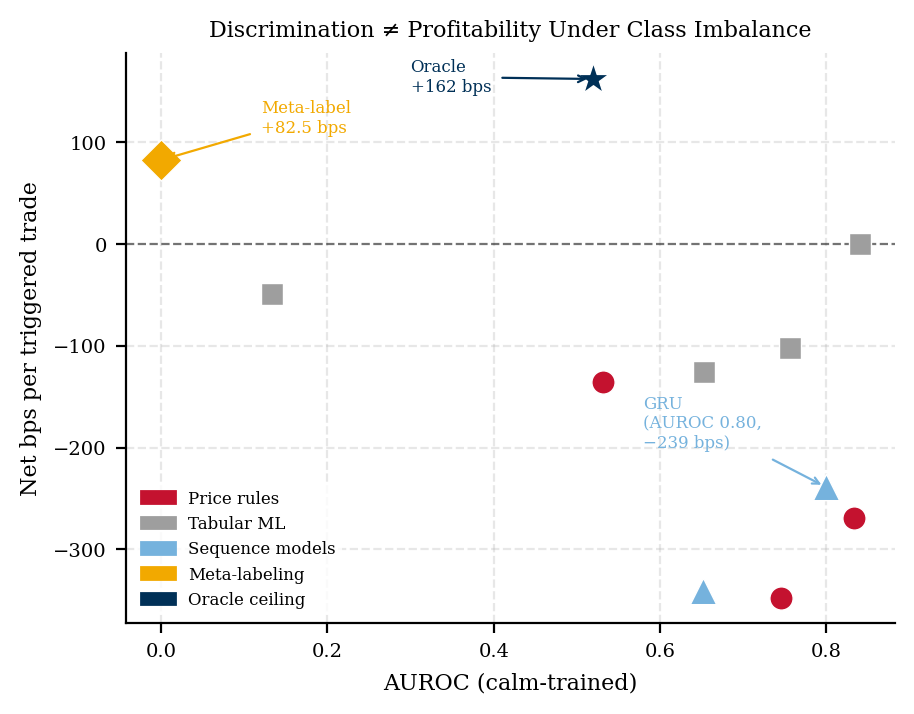
\includegraphics[width=\columnwidth]{../results/paper/figures/figure_auroc_pnl_scatter.png}
  \caption{AUROC vs.\ net bps for calm-trained models on the SVB test split. Models cluster
    in the upper left: high discrimination, negative P\&L. The GRU (AUROC~0.80, $-239\bps$) is
    annotated to illustrate the inversion---no threshold isolates the $2.88\%$ executable
    minority. Oracle (navy star) is the achievable ceiling.}
  \label{fig:auroc_pnl}
\end{figure}

\begin{table}[t]
\centering
\caption{Tabular model ladder (\task{basis\_usdc\_1m\_gt10bps}).
  Hit\% is fraction of executable trades.
  $^\dagger$Oracle ceiling. $^\ast$0-trade degenerate.}
\label{tab:ablation}
\setlength{\tabcolsep}{2pt}
{\scriptsize
\begin{tabular}{lrrrrr}
\toprule
\textbf{Model} & \textbf{Feat.} &
\textbf{Net\,bps} & \textbf{Trades} & \textbf{AUROC} & \textbf{Hit\%}\\
\midrule
Oracle$^\dagger$ & --  & $+161.7$ & 316  & --   & 100\%\\
\midrule
\texttt{lgbm}$^\ast$    & all  & --      & 0    & 0.653 & --\\
\texttt{logistic}       & all  & $-49.1$  & 1    & 0.133 &  0\%\\
\texttt{gross\_arb}     & px   & $-136.0$ & 611  & 0.531 &  4\%\\
\texttt{price\_10}      & px   & $-269.5$ & 2002 & 0.833 &  6\%\\
\texttt{price\_25}      & px   & $-347.3$ & 1025 & 0.746 &  5\%\\
\texttt{no\_trade}      & --  & $\phantom{-}0.0$  & 0    & --   & --\\
\midrule
\texttt{ExpNet\_lgbm}   & px   & $-73.8$  & 537  & --   &  6\%\\
\texttt{ExpNet\_xgb}    & px   & $-57.2$  &  70  & --   &  9\%\\
\midrule
\texttt{lgbm\_weighted} & pb   & $-65.9$  &   2  & 0.497 &  0\%\\
\texttt{xgb\_weighted}  & px   & $-90.5$  &  30  & 0.631 &  0\%\\
\texttt{rf\_balanced}   & px   & $-89.2$  &  11  & 0.467 &  0\%\\
\bottomrule
\multicolumn{6}{l}{\footnotesize px\,=\,\texttt{price\_only},
  pb\,=\,\texttt{price\_plus\_book},
  all\,=\,\texttt{price\_book\_settle}.}\\
\end{tabular}
}
\end{table}

\begin{figure}[t]
  \centering
  \includegraphics[width=\columnwidth]{../results/paper/figures/figure_oracle_gap_waterfall.png}
  \caption{Oracle gap decomposition (\$10K notional, SVB test split).
    False-positive drag (the mean net loss on trades flagged positive but not
    executable) is directly measured. Timing error (40--80\,bps) and sizing
    error (40--100\,bps) are estimated from entry-delay and notional-scaling
    analysis.}
  \label{fig:waterfall}
\end{figure}

Figure~\ref{fig:waterfall} decomposes the 260\,bps oracle gap into false-positive
drag (dominant), timing error ($40$--$80\bps$), and sizing error ($40$--$100\bps$).


\subsection{Executable-Window Selection: Unsolved on CEX, Profitable On-Chain}
\label{sec:diagnostics}

\paragraph{What does not work (CEX).} Can \emph{any} model select the profitable executable
windows among optical fires? We answer with a pre-registered grid search over training
protocol $\times$ feature set $\times$ model, scored out-of-sample on the SVB execution-grade
split. Protocols are cross-mechanism (train Terra/LUNA $\to$ test SVB), calm-control $\to$ SVB,
in-event walk-forward (train first-half SVB $\to$ test second-half), and a purged five-fold
in-event cross-validation (embargoed)---the easiest possible setting, train and test within the
\emph{same} crisis. Feature sets are price-only, price-plus-book, and book-dynamics (adding
depth-withdrawal velocity and basis/spread deltas); models are LightGBM
meta-labeling~\cite{lopezdeprado2018}, logistic regression, and random forests, at
\$10k/\$50k/\$100k notionals. Every decision threshold is calibrated on the \emph{training}
segment only. Across \textbf{81 logged paths, zero} clear a Benjamini--Hochberg FDR($0.10$)
gate~\cite{benjamini1995fdr} on (net bps${>}0$, bootstrap $95\%$ CI lower bound${>}0$,
$n{\ge}30$): the best single path returns $+7.7\bps$ but with CI $[-23,+41]$ (not significant),
and the mean cross-mechanism path is $-28\bps$. Decisively, even the purged in-event CV is
strongly negative ($-66$ to $-122\bps$): the profitable minority is \emph{unpredictable from
this microstructure}, not merely non-transferable. Selecting executable windows on the CEX
order book is, on this data, unsolved---a standing challenge the benchmark poses.

\begin{table}[h]
\centering
\caption{The CEX selection null is robust: mean out-of-sample net bps by training protocol over the
  $81$-path pre-registered search (well-defined paths, $n{\ge}30$). No protocol is profitable, and
  even purged in-event cross-validation---the easiest setting, train and test \emph{within} SVB---is
  strongly negative. Best single path: cross-mechanism logistic, $+7.7\bps$, $95\%$ CI $[-23,+41]$
  (not significant).}
\label{tab:cexnull}
\setlength{\tabcolsep}{5pt}
{\small
\begin{tabular}{lrl}
\toprule
\textbf{Training protocol} & \textbf{Mean net bps} & \textbf{Setting} \\
\midrule
Cross-mechanism (Terra$\to$SVB)    & $-28$ & hardest (transfer) \\
Purged in-event CV (within SVB)    & $-75$ & easiest (in-distribution) \\
In-event walk-forward (within SVB) & $-94$ & in-distribution \\
\bottomrule
\multicolumn{3}{@{}p{0.92\columnwidth}@{}}{\footnotesize $0/81$ paths clear the Benjamini--Hochberg
  FDR($0.10$) gate (net${>}0$, bootstrap CI${>}0$, $n{\ge}30$). Grid: feature sets
  \{price-only, price-plus-book, book-dynamics\} $\times$ models \{LightGBM meta-label, logistic,
  random forest\} $\times$ notionals \{\$10k,\$50k,\$100k\}.}\\
\end{tabular}
}
\end{table}

\paragraph{What does work (on-chain).} The barrier is venue-specific. We repeat the test on the
\emph{real} on-chain Curve/AMM panel ($4{,}994$ rows across five episodes, \S\ref{sec:venue}),
where the capturable dislocation is $\text{net}=|\text{basis}|-\text{slippage}_{10k}-\text{fee}$,
the benchmark's own AMM-executable formula (single-leg, $1\bps$ Curve StableSwap
fee~\cite{egorov2019stableswap}). Because pool slippage is bounded and small (median
$0.8$--$5.5\bps$), a \emph{model-free} deviation rule (capture every optical fire) is profitable
in $5/5$ episodes (Table~\ref{tab:onchain}). Under a deliberately conservative $30\bps$ gas
haircut---per-row gas is absent from the source panel, so we charge a fixed cost equivalent to a
$\sim\!\$30$ swap on a $\$10k$ notional, above the $2022$--$23$ median---$4/5$ episodes remain
robustly profitable ($+169$ to $+463\bps$, moving-block bootstrap~\cite{politis1994stationary}
$95\%$ CIs above zero); the lone failure is the small USDC/SVB on-chain dislocation
($+9.4\bps$ pre-gas). The \emph{same} deviation signal that loses money on every CEX path is
capturable on-chain (Figure~\ref{fig:venue}).

\begin{table}[h]
\centering
\caption{On-chain executable arbitrage: a model-free deviation rule (capture optical fires,
  $|\text{basis}|{>}10\bps$) on real Curve/AMM pool data. Net bps per trade, moving-block
  bootstrap $95\%$ CI (block${=}30$); ``$-30\bps$ gas'' subtracts a fixed conservative swap-gas
  cost (stated assumption; per-row gas absent in source).}
\label{tab:onchain}
\setlength{\tabcolsep}{4pt}
{\small
\begin{tabular}{lrrr}
\toprule
\textbf{Episode} & \textbf{Net bps} & \textbf{$-30\bps$ gas} & \textbf{$n$} \\
\midrule
USDT/Curve (Jun 2023) & $+371$ & $+341$ & 697 \\
Terra/LUNA (May 2022) & $+381$ & $+351$ & 549 \\
FTX (Nov 2022)        & $+493$ & $+463$ & 353 \\
BUSD (Feb 2023)       & $+199$ & $+169$ & 766 \\
USDC/SVB (Mar 2023)   & $+9.4$ & $-21$  & 375 \\
\bottomrule
\multicolumn{4}{@{}p{0.92\columnwidth}@{}}{\footnotesize All five CIs exclude zero pre-gas; four
  of five remain above zero after the gas haircut. Contrast: the identical signal yields $0/81$
  profitable paths on the CEX order book.}\\
\end{tabular}
}
\end{table}

\begin{figure*}[t]
  \centering
  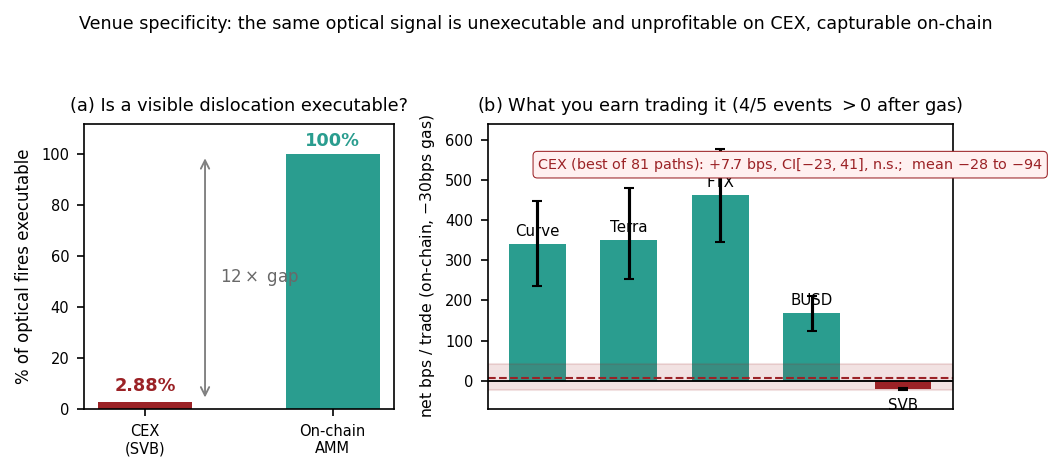
\includegraphics[width=0.86\textwidth]{../results/paper/figures/figure_venue_specificity.png}
  \caption{Venue specificity in one view. \textbf{(a)}~Of the optically dislocated minutes, only
    $2.88\%$ are executable on the CEX order book versus $100\%$ on the on-chain Curve/AMM pool---a
    $12\times$ gap. \textbf{(b)}~Trading those windows, a model-free deviation rule earns $+169$ to
    $+463\bps$ on-chain in four of five episodes after a conservative $30\bps$ gas haircut
    (moving-block bootstrap $95\%$ CIs shown); the lone exception is the small USDC/SVB dislocation.
    On the CEX order book the same signal yields $0/81$ profitable paths (best $+7.7\bps$, CI
    $[-23,+41]$, n.s.; protocol means $-28$ to $-94\bps$). The optical-to-executable barrier is a
    property of CEX order-book microstructure, not of stablecoin depegs.}
  \label{fig:venue}
\end{figure*}

\paragraph{Why.} On a CEX, capturing a visible dislocation means walking a thin, fee-laden book
with settlement delay, so most optical fires are not executable and which ones are cannot be
predicted ahead of time. On an automated market maker, execution cost is the deterministic
slippage of the pool invariant, so a visible dislocation above the fire threshold is almost
always a real, capturable one. The lesson for execution-aware AI is that the venue's
microstructure, not the crisis mechanism, decides whether a learned signal is tradeable.

\paragraph{Why these choices.} Each parameter is fixed by a prior or a stated rationale, not tuned to a
result. The $10\bps$ optical-fire threshold matches the CEX primary-signal pipeline used throughout the
benchmark, so the on-chain and CEX tests fire on the same definition. The $1\bps$ swap fee is Curve's
StableSwap pool fee~\cite{egorov2019stableswap}. Because per-row gas is absent from the on-chain panel we
do not infer it from a volatile gas series; we instead charge a fixed $30\bps$ haircut---equivalent to a
$\sim\!\$30$ swap on a \$10k notional, above the $2022$--$23$ median Curve-swap cost---so the on-chain
result is reported under a deliberately pessimistic execution assumption, and we report the pre-gas figure
alongside it. Significance uses a moving-block bootstrap (block $=30$ minutes)~\cite{politis1994stationary}
because per-minute returns within an event are serially correlated, and a finding must additionally clear a
Benjamini--Hochberg FDR($0.10$) gate~\cite{benjamini1995fdr} across the whole ledger, so searching many
paths cannot manufacture a false positive. Every decision threshold is calibrated on the training segment
only; no result uses the test split for tuning.



\section{Limitations}
\label{sec:limitations}
\paragraph{Scope.}
The negative CEX result is a finding, not a sample-count artefact: it spans 81 pre-registered
paths and is strongest precisely where data is most plentiful (in-distribution purged CV). Three
honest limits remain.
\textbf{(1)~Single execution-grade CEX destination.} A second Tier-A CEX pair is unavailable
(Binance's pre-2024 archive lacks L2 depth), so the $12{\times}$ gap is measured on SVB; the
five-event on-chain AMM result (all ${\approx}1{\times}$) is the cross-event evidence that the
barrier is CEX-specific.
\textbf{(2)~Proxy buy leg.} The SVB CEX gap uses a kline-proxy BTC-USDC buy leg; a $20\%$
haircut bounds it to $12$--$14{\times}$ with the oracle still above $+130\bps$.
\textbf{(3)~Stylised on-chain execution.} The on-chain net uses the pool-invariant slippage at
\$10k and a single-leg $1\bps$ fee, with gas charged as a fixed conservative $30\bps$ haircut
(per-row gas is absent from the panel); it omits MEV competition, which would erode---but, given
the $+169$ to $+463\bps$ margins, is unlikely to erase---the on-chain edge on the large dislocations.

%% =============================================================
\section{Conclusion}
\label{sec:conclusion}

Price-label benchmarks measure the wrong object: $34.3\%$ of SVB minutes appeared
dislocated but only $2.88\%$ survived VWAP execution (a $12\times$ gap). StressBench scores
models by oracle capture instead, and the result is two-sided. \emph{On the CEX order book the
problem is unsolved}: no calm-trained family is profitable, AUROC is anti-correlated with P\&L,
and a pre-registered 81-path search finds nothing that survives FDR correction---even
in-distribution. \emph{On-chain the same dislocation is tradeable}: a model-free deviation rule
earns $+169$ to $+463\bps$ in four of five episodes after a conservative gas haircut, because
pool slippage is bounded. The optical-to-executable barrier is therefore a property of CEX
microstructure, not of depegs.
\textbf{Practitioner rules:}
(1)~Divide every price-label AUROC by the venue's execution gap before any capital decision.
(2)~On a CEX, treat executable-window selection as an open problem, not a solved one.
(3)~For execution-aware capture, the on-chain venue---not a cleverer model---is what makes the
signal tradeable.
Future work: a second Tier-A CEX event, an MEV-aware on-chain execution model, and early-entry
timing labels.

\section*{Acknowledgements}
Code and data available at anonymized repository (link at camera-ready).

%% =============================================================
\bibliographystyle{ACM-Reference-Format}
\scriptsize
\begin{thebibliography}{23}
\setlength{\itemsep}{1pt plus 0.2ex}

\bibitem{uhlig2022luna}
Uhlig, H.\ (2022).
\newblock A Luna-tic stablecoin crash.
\newblock {\em NBER Working Paper 30256}.

\bibitem{griffin2020tether}
Griffin, J.~M. and Shams, A.\ (2020).
\newblock Is Bitcoin really untethered?
\newblock {\em Journal of Finance}, 75(4):1913--1964.

\bibitem{hautsch2018blockchain}
Hautsch, N. Scheuch, C. and Voigt, S.\ (2018).
\newblock Building trust takes time. Limits to arbitrage for blockchain-based
  assets.
\newblock {\em arXiv:1812.00595}.

\bibitem{shleifer1997limits}
Shleifer, A. and Vishny, R.~W.\ (1997).
\newblock The limits of arbitrage.
\newblock {\em Journal of Finance}, 52(1):35--55.

\bibitem{gromb2010limits}
Gromb, D. and Vayanos, D.\ (2010).
\newblock Limits of arbitrage. The state of the theory.
\newblock {\em Annual Review of Financial Economics}, 2:251--275.

\bibitem{cont2013optimal}
Cont, R. and Kukanov, A.\ (2013).
\newblock Optimal order placement in limit order markets.
\newblock {\em Quantitative Finance}, 17(1):21--39.

\bibitem{makarov2020trading}
Makarov, I. and Schoar, A.\ (2020).
\newblock Trading and arbitrage in cryptocurrency markets.
\newblock {\em Journal of Financial Economics}, 135(2):293--319.

\bibitem{lopezdeprado2018}
L\'{o}pez de Prado, M.\ (2018).
\newblock {\em Advances in Financial Machine Learning}.
\newblock Wiley.

\bibitem{cintra2023bocpd}
Cintra, R. and Holloway, C.\ (2023).
\newblock Detecting depegs. Towards safer passive liquidity provision on
  Curve Finance.
\newblock {\em arXiv:2306.10612}.

\bibitem{vidalthomas2023ftx}
Vidal-Tom\`{a}s, D. Briola, A. and Aste, T.\ (2023).
\newblock FTX's downfall and Binance's consolidation.
\newblock {\em arXiv:2302.11371}.

\bibitem{gatev2006pairs}
Gatev, E. Goetzmann, W.~N. and Rouwenhorst, K.~G.\ (2006).
\newblock Pairs trading. Performance of a relative-value arbitrage rule.
\newblock {\em Review of Financial Studies}, 19(3):797--827.

\bibitem{tibshirani1996lasso}
Tibshirani, R.\ (1996).
\newblock Regression shrinkage and selection via the lasso.
\newblock {\em JRSS-B}, 58(1):267--288.

\bibitem{breiman2001random}
Breiman, L.\ (2001).
\newblock Random forests.
\newblock {\em Machine Learning}, 45(1):5--32.

\bibitem{chen2016xgboost}
Chen, T. and Guestrin, C.\ (2016).
\newblock XGBoost. A scalable tree boosting system.
\newblock In {\em KDD}, pp.~785--794.

\bibitem{adamsmackay2007bocpd}
Adams, R.~P. and MacKay, D.~J.~C.\ (2007).
\newblock Bayesian online changepoint detection.
\newblock {\em arXiv:0710.3742}.

\bibitem{moallemi2022rl}
Moallemi, C.~C. and Wang, M.\ (2022).
\newblock A reinforcement learning approach to optimal execution.
\newblock {\em Quantitative Finance}, 22(6):1051--1069.

\bibitem{ning2021ddql}
Ning, B. Lin, F.~H.~T. and Jaimungal, S.\ (2021).
\newblock Double deep Q-learning for optimal execution.
\newblock {\em Applied Mathematical Finance}, 28(4):361--380.

\bibitem{gogol2024amm}
Gogol, K. Messias, J. Miori, D. Tessone, C. and Livshits, B.\ (2024).
\newblock Quantifying arbitrage in automated market makers. An empirical study
  of {Ethereum} {ZK} rollups.
\newblock In {\em MARBLE 2024}.

\bibitem{adams2023mev}
Adams, A. Chan, B.~Y. Markovich, S. and Wan, X.\ (2023).
\newblock Don't let {MEV} slip. The costs of swapping on the {Uniswap}
  protocol.
\newblock {\em arXiv:2309.13648}.

\bibitem{hernandezcruz2024svb}
Hernandez~Cruz, W. Xu, J. Tasca, P. and Campajola, C.\ (2024).
\newblock No questions asked. Effects of transparency on stablecoin liquidity
  during the collapse of {Silicon Valley Bank}.
\newblock {\em arXiv:2407.11716}.

\bibitem{jaxmarlhft2024}
Mohl, V. Frey, S. Leyland, R. Li, K. Nigmatulin, G. Cucuringu, M.
  Zohren, S. Foerster, J. and Calinescu, A.\ (2025).
\newblock {JaxMARL-HFT}. {GPU}-accelerated large-scale multi-agent
  reinforcement learning for high-frequency trading.
\newblock In {\em ICAIF '25}. ArXiv:2511.02136.

\bibitem{rightplace2024}
Olby, O. Bacalum, A. Baggott, R. and Stillman, N.\ (2025).
\newblock Right place, right time. Market simulation-based {RL} for execution
  optimisation.
\newblock In {\em ICAIF '25}. ArXiv:2510.22206.

\bibitem{benjamini1995fdr}
Benjamini, Y. and Hochberg, Y.\ (1995).
\newblock Controlling the false discovery rate: a practical and powerful approach to multiple
  testing.
\newblock {\em Journal of the Royal Statistical Society: Series B}, 57(1):289--300.

\bibitem{politis1994stationary}
Politis, D.N. and Romano, J.P.\ (1994).
\newblock The stationary bootstrap.
\newblock {\em Journal of the American Statistical Association}, 89(428):1303--1313.

\bibitem{egorov2019stableswap}
Egorov, M.\ (2019).
\newblock StableSwap: efficient mechanism for stablecoin liquidity.
\newblock Curve Finance whitepaper.

\bibitem{iaqf_uchicago_crosscurrency_2026}
Kohli, D., Yadav, S., Agarwal, S., and Bhaskara, P.\ (2026).
\newblock Cross-Currency Dynamics in Cryptocurrencies under Stablecoin Regulation.
\newblock {\em 15th Annual IAQF Academic Affiliate Student Competition} (University of Chicago, ``Inefficient Markets'').

\bibitem{iaqf_nyu_spread_2026}
Kakumani, R., Andersen, J., Zhong, J., Agarwal, A., Lam, H., and Tomar, H.\ (2026).
\newblock Cross-Currency Dynamics in Cryptocurrencies under Stablecoin Regulation.
\newblock {\em 15th Annual IAQF Academic Affiliate Student Competition} (New York University, ``Spread Hunters'').

\end{thebibliography}

\end{document}
